\chapter{Psalm 30}

\begin{figure}
  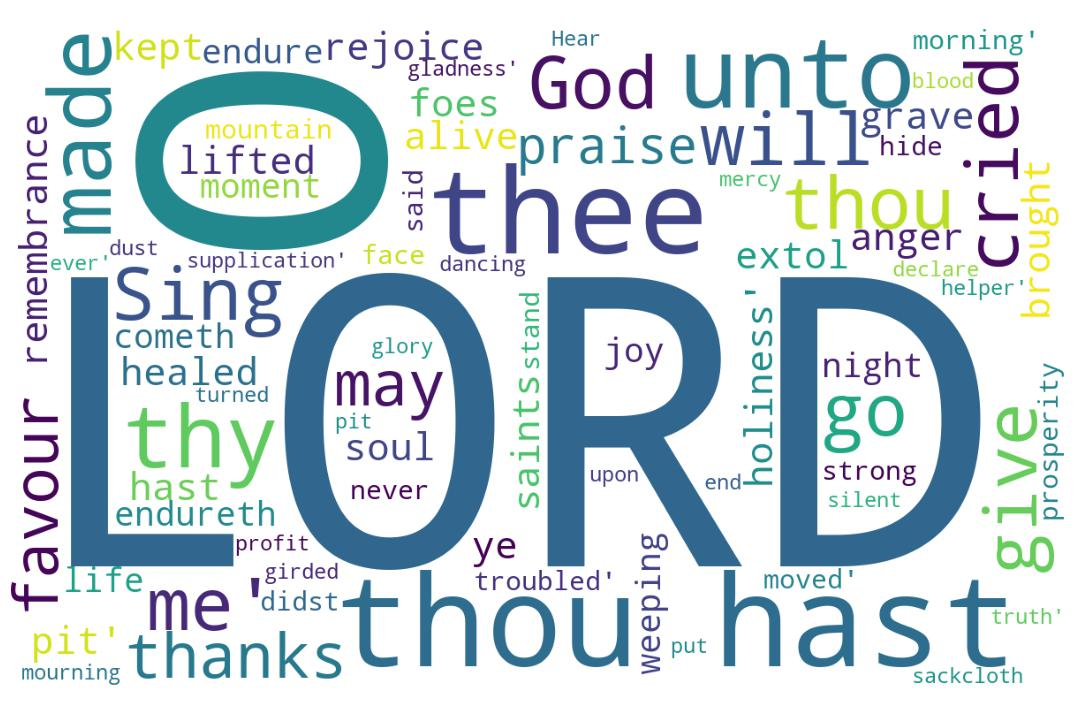
\includegraphics[width=\linewidth]{19OT-Psalms/Psalm30-WordCloud.jpg}
  \caption{Psalm 30 Word Cloud}
  \label{fig:Psalm 30 word Cloud}
\end{figure}
%%%%%%%%%%%%%%%%%%%%%%%%%%%%%%%%%%%%%%%%%
%%%%%%%%%%%%%%%%%%%%%%%%%%%%%%%%%%%%%%%%%

\marginpar{\scriptsize \centering \fcolorbox{bone}{lime}{\textbf{GOD'S FAVOUR}}\\ (Psalm 30:1--12) 
\begin{compactenum}[I.][8]
    \item David spared at the \textbf{Brink of Death} \index[scripture]{Psalms!Psa 030:03} (Psa 30:3)
    \item God's favor was David's \textbf{Basis for Deliverance} \index[scripture]{Psalms!Psa 030:05} (Psa 30:5)
    \item David's \textbf{Bad Declaration} \index[scripture]{Psalms!Psa 030:06} (Psa 30:6)
    \item David's \textbf{Better Decision}  \index[scripture]{Psalms!Psa 030:07} (Psa 30:7)
    \item David gets \textbf{Blessing instead of Dust} \index[scripture]{Psalms!Psa 030:09} (Psa 30:9)
    \item God changed David's \textbf{Bitterness into Dancing} \index[scripture]{Psalms!Psa 030:11} (Psa 30:11)
    \item David gets a \textbf{Bright Destiny} \index[scripture]{Psalms!Psa 030:12} (Psa 30:12)
\end{compactenum} }

\footnote{\textcolor[cmyk]{0.99998,1,0,0}{\hyperlink{TOC}{Return to end of Table of Contents.}}}\footnote{\href{https://www.audioverse.org/english/audiobibles/books/ENGKJV/O/Ps/1}{\textcolor[cmyk]{0.99998,1,0,0}{Psalms Audio}}}\textcolor[cmyk]{0.99998,1,0,0}{A Psalm \emph{and} Song \emph{at} the dedication of the house of David.}\\
\\
\textcolor[cmyk]{0.99998,1,0,0}{I will extol thee, O LORD; for thou hast lifted me up, and hast not made my foes to rejoice over me.}
[2] \textcolor[cmyk]{0.99998,1,0,0}{O LORD my God, I cried unto thee, and thou hast healed me.}
[3] \textcolor[cmyk]{0.99998,1,0,0}{O LORD, thou hast brought up my soul \fcolorbox{bone}{lime}{from the grave}: thou hast kept me alive, that I should not go down to the pit.}
[4] \textcolor[cmyk]{0.99998,1,0,0}{Sing unto the LORD, O ye saints of his, and give thanks at the remembrance of his holiness.}
[5] \textcolor[cmyk]{0.99998,1,0,0}{For his anger \emph{endureth} \emph{but} a moment; in \fcolorbox{bone}{lime}{his favour} \emph{is} life: weeping may endure for a night, but joy \emph{cometh} in the morning.}
[6] \textcolor[cmyk]{0.99998,1,0,0}{And in my prosperity I said, I shall \fcolorbox{bone}{lime}{never} be moved.}
[7] \textcolor[cmyk]{0.99998,1,0,0}{LORD, by \fcolorbox{bone}{lime}{thy favour} thou hast made my mountain to stand strong: thou didst hide thy face, \emph{and} I was troubled.}
[8] \textcolor[cmyk]{0.99998,1,0,0}{I \fcolorbox{bone}{lime}{cried to thee}, O LORD; and unto the LORD I made supplication.}
[9] \textcolor[cmyk]{0.99998,1,0,0}{What profit \emph{is} \emph{there} in my blood, when I go down to the pit? Shall the \fcolorbox{bone}{lime}{dust} praise thee? shall it declare thy truth?}
[10] \textcolor[cmyk]{0.99998,1,0,0}{Hear, O LORD, and have mercy upon me: LORD, be thou my helper.}
[11] \textcolor[cmyk]{0.99998,1,0,0}{Thou hast turned for me my mourning into \fcolorbox{bone}{lime}{dancing}: thou hast put off my sackcloth, and girded me with gladness;}
[12] \textcolor[cmyk]{0.99998,1,0,0}{To \fcolorbox{bone}{lime}{the end} that \emph{my} glory may sing praise to thee, and not be silent. O LORD my God, I will give thanks unto thee for ever.}